\subsection{Dokumenten-Management-Systeme}

Um ein Dokumenten-Management-System (\gls{DMS})  zu erläutern muss sich zuerst mit dem Begriff des \textbf{"`Dokuments"'} auseinander gesetzt werden.
In \cite{DMS08} S. 2 wird ein Dokument durch folgende Punkte definiert:

\begin{itemize}
\item Ein Dokument fasst inhaltlich zusammengehörende Informationen strukturiert zusammen, die nicht ohne erheblichen Bedeutungsverlust weiter unterteilt werden können. 
\item Die Gesamtheit der Information ist für einen gewissen Zeitraum zu erhalten.
\item Dokumente dienen oft dem Nachweis von Tatsachen.
\item Ein Dokument ist als Einheit ablegbar (speicherbar) und/oder versendbar und/oder wahrnehmbar (sehen, hören, fühlen).
\item Das Dokument ist eigentlich der Träger, der die Informationen speichert, egal ob das Dokument ein Stück Paper, eine Datei auf einem Rechner, ein Videoband oder eine Tontafel etc. ist. Dies bedeutet auch, dass es keine Bindung an Papier oder ein geschriebenes Wort gibt.
\end{itemize}

Desweiteren gibt es eine Differenzierung in zwei Definitionen:

\begin{quote}"`Als \textbf{Dokument im konventionellen Sinne} werden Dokumente bezeichnet, die als körperliches Dokumente (z. B. Papier) vorliegen, ursprünglich als körperliches Dokument vorlagen oder für die Publizierung auf einem körperlichen Medium vorgesehen sind.

Die Begrifflichkeit des \textbf{Dokuments im weiteren Sinne} erweitert den Begriff des Dokuments um semantisch zusammengehörende Informationsbestände , die für die Publikation in nicht-körperlichen Medien, z. B. Webseiten, Radio, Fernsehen o. ä. vorgesehen sind. Derartige Dokumente werden oft dynamisch gestaltet und zusammengestellt."' \begin{flushright}\cite{DMS08} S. 2\end{flushright}\end{quote}

Unter \textbf{Dokumenten-Management} werden primär die Verwaltungsfunktionen Erfassung, Bearbeitung, Verwaltung und Speicherung von Dokumenten verstanden. \cite{DMS08} S. 344.

Darunter fallen laut \cite{DMS08} S. 3 folgende Punkte:

\begin{itemize}
\item Kennzeichnung und Beschreibung von Dokumenten (auch Metadaten des Dokuments genannt) 
\item Fortschreibung, Versionierung und Historienverwaltung von Dokumenten
\item Ablage und Archivierung von Dokumenten
\item Verteilung und Umlauf von Dokumenten
\item Suche nach Dokumenten bzw. Dokumenteninhalten
\item Schutz der Dokumente vor Verfälschung, Missbrauch und Vernichtung
\item Langfristiger Zugriff auf die Dokumente und Lesbarkeit der Dokumente
\item Lebenslauf und Vernichtung von Dokumenten
\item Regelung von Verantwortlichkeiten für Inhalt und Verwaltung von Dokumenten
\end{itemize}

Der Begriff \textbf{"`Dokumenten-Management-System"'} muss auch in zwei verschiedene Sichtweisen differenziert werden:
\begin{quote}"`Bei \textbf{Dokumenten-Management-Systemen im engeren Sinne} geht es um die Logik der Verwaltung von Dokumenten, deren Status, Struktur, Lebenzyklus und Inhalt. Dokumente werden beschrieben, klassifiziert und in einer bestimmten logischen Struktur eingeordnet, damit sie einfach wieder gefunden werden können. Dokumente entstehen, werden verändert und (irgendwann) vernichtet.

Den \textbf{Dokumenten-Management-Systemen im weiteren Sinne} ordnet man auch noch weitere Funktionalitäten zu, wie z. B. Schrifterkennung, automatische Indizierung, [...], Publizierung. Hier lassen sich die Grenzen nicht mehr genau bestimmten!"' \begin{flushright}\cite{DMS08} S. 5\end{flushright}\end{quote}

\subsection{Content-Management-Systeme}
Bei einem Content-Management-System (\gls{CMS})  steht nicht mehr das eigentliche Dokument im Vordergrund, sondern vielmehr der enthaltene Informationsgehalt des Dokuments.
Der Unterschied zwischen einem DMS und einem CMS besteht laut \cite{DMS08} S. 114 im/in Folgenden/m:

\begin{quote}"`Abgrenzend zum Dokumenten-Management handelt es sich beim Content-Management nicht vordergründig um die Verwaltung von Dokumenten, sondern um die Verwaltung von Informationseinheiten, die miteinander verknüpft sein können. [...] Je nach ausprägung kann nun ein konkretes System als Dokumenten-Management-System mit Content-Management-Funktionen definiert werden und umgekehrt. [...]
Der Ansatz des Content-Management unterscheidet sich vom "`klassischen"' Dokumenten-Mangement vor allem in Bezug auf die betrachteten Objekte: Ein DMS hat als kleinestes Objekt der Betrachtung eines einzelnen Dokument. [...] Content-Management ist auf logische Informationseinheiten ausgerichtet. Es ist z.B. das Ziel des Content-Managements, Inhalte, die auf mehrere Quellen verteilt sind, neue zusammenzustellen und daraus z.B. ein neues Dokument zu generieren."'
\begin{flushright}\cite{DMS08} S. 114f\end{flushright}\end{quote}

Die folgende Abbildung soll den (charakteristischen) Unterschied zwischen CMS-Systemen und DMS-Systemen verdeutlichen.

\begin{center}
Bild \cite{DMS08} S. 115
\end{center}

Wie zuvor beschrieben ist die Sichtweise eines DMS nur auf die einzelnen Dokumente beschränkt, während ein CMS einzelne Elemente / Informationen aus den Dokumenten extrahieren und daraus ggf. ein neues Dokument generieren kann. Die Sichtweise des CMS wird durch das gestrichelte Polygon dargestellt, welches hier dokumentenübergreifend abgebildet ist.

Der (theoretische/beabsichtigte) Zweck, weshalb ein CMS-System eingesetzt wird, ist laut Oracle folgendermaßen definiert:

\begin{quote}"`The key to a successful content management implementation is unlocking the value of content by making it as easy as possible for it to be consumed. This means that any piece of content must be available to any consumer, no matter what their method of access."'
\begin{flushright}\cite{UCM07} S. 12\end{flushright}\end{quote}

Ein CMS soll die Informationen jedes/jedwedem (Inhalts) extrahieren/aufnehmen und jedes Einzelteil / Element dieser Information den Benutzern zugänglich machen, unabhängig von der Art des Zugriffs.
Dieses Konzept soll in Abbildung \ref{ucm-a2a} verdeutlicht werden.

\begin{figure}[ht]
	\centering
	   \fbox{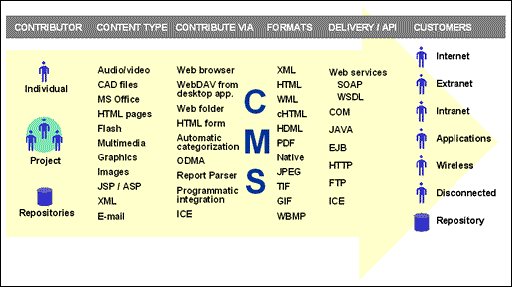
\includegraphics[width=0.95\textwidth]{bilder/ucm.png}}
		\caption["`any-to-any"' Content-Management Konzept]{"`any-to-any"' Content-Management Konzept\protect\footnote}
		\label{ucm-a2a}
\end{figure}
\footnotetext{Quelle: \cite{UCM07} S. 12}

Das CMS steht hier in der Mitte der Abbildung als Medium zwischen den verschiedenen Inhalten, eingestellt von den \textit{Contributors} (links), und den Anwendern, die auf transformierte Versionen der Inhalte durch unterschiedliche Arten zugreifen (rechts).


\subsection{Enterprise-Content-Management-Systeme - optional}
In diesem Zusammenhang / Kontext sei auch der Begriff Enterprise-Content-Management (\gls{ECM}) genannt.
Laut der "`Association for Information and Image Management"' (\gls{AIIM}\footnote{Die AIIM ist eine Gesellschaft von internationalen Herstellern und Anwendern von Informations- und Dokumenten-Mangement-Systemen}), welche sich mit umfasst dieser Begriff die Verwaltungfunktionen von Unternehmensinformationen in unterschiedlichen Dokumentformaten.\footnote{Quelle: \url{http://www.aiim.org/What-is-ECM-Enterprise-Content-Management.aspx}}
Diese Funktionen werden laut \cite{DMS08} S. 116 durch verschiedene "`Systeme wie Dokumenten-Management, Groupware, Workflow, Input- und Output-Management, (Web-)Content-management, Archivierung, Records-Management und andere"' bereitsgestellt.


\subsection{Universal-Content-Management-Systeme}

























